% !TeX root = ../report.tex

\section{User Testing}
\subsection{Method}
%General method (what is UT)
%Copy and past of definition

User Testing is a methodology aimed at evaluating the usability of an application, where by "usability" we mean "the effectiveness, efficiency and satisfaction with which specified users can achieve specified goals in particular environments" (ISO 9241-11). Therefore, User Testing is a task-oriented empirical research which involves end users that are observed by researchers while the former are using the application.

\subsection{Design of the study}
    The user testing was performed both remotely and in-presence, with the use of two personal computers, one for the end user and one for the evaluator.\\
    In case of an remote approach, the users were asked to share their screen via a videoconferencing software to let the evaluator observe their actions.

    \subsubsection{User profile and recruitment}
    % Explain the two different user profiles
    For our analysis, we selected two User Profiles:

    \begin{itemize}
        \item College students that live in Milan 
        \item Tourists that wants to visit the city
    \end{itemize}

    Both the user profiles were selected between the age of 20 and 30 years old.\\
    For the recruitment, each evaluator has recruited 5 users between friends or relatives of the evaluator, for a total of 20 users.

    \subsubsection{Metrics and indicators}
    Both quantitative and qualitative indicators were measured.\\
    The quantitative indicators are:
    \begin{itemize}
        \item Effectiveness or task success rate. We assigned 1 point if the user has successfully completed the task, without requiring any assistance; 0.5 points if the user was able to complete the task, but requesting the examiner's assistance for one or more steps; 0 points if the user has given up, or has thought he has finished when he has not.
        \item Efficiency, measured by the time (in minutes and seconds) taken by the user to complete the task.
        \item Errors, which corresponds to the number of wrong paths or actions taken by the user while completing the task.
        \item Perceived tasks difficulty, measured by asking the user to assign a score from 1 (very easy)  to 5 (impossible).
    \end{itemize}
    
    Whereas for qualitative indicators, we collected short textual descriptions of how the user was performing during the task.

    \subsubsection{Tasks}
    % Tasks list
    % Explain that for each different user profile different task
    We have defined 6 tasks per user profile, so as to further analyze the most relevant sections of the site that we had already inspected in the inspection phase.

    Although the tasks assigned to each user profile have been defined according to the importance for the specific user, some tasks overlap because they are interesting for both user profiles.

    The site has both simple and complex features so we have defined both simple and complex tasks, to simulate the experience of a real user.
    
    For the user profile ``college students that live in Milan'' we defined the following tasks:

    \begin{enumerate}
        
        \item You are a design student at polimi. You want to see what are the major art events of the year, in particular look for the triennale.
        \item You are considering which university to enroll to. Try to find out which are the universities in Milan that offer a bachelor degree in economics as an Exchange/International Student.
        \item You are an exchange student from US, and you will rent a house here at Milan. Find the required documents to sign a tenancy contract.
        \item You want to move around and orient yourself in Milan. Find information and download the map about public transports.
        \item You are interested in visiting Milano, but you are unsure of the covid situation of the city and its policies (e.g. regarding green pass). Find more about it and where to get tested.
        \item You want to find the list of museums in Milano whose entrance is free. Select the first and look for its opening times, how to reach it and if there are any parking spots. 
    \end{enumerate}
        For the user profile "tourists that wants to visit the city" we defined the following tasks:
    \begin{enumerate}
        \item For this saturday, you've planned to shop at Porta Venezia till lunch time. Find and book the nearest restaurant in the area for that saturday, in particular you are a vegan.
        \item You are planning to book an hotel near the city center (Duomo) for the weekend for two adults, a child and your lovely dog.
        \item You are a tourist with three free days, search a suitable itinerary in Milan that may last from one up to three days.
        \item You want to move around and orient yourself in Milan. Find information and download the map about public transports.
        \item You are interested in visiting Milano, but you are unsure of the COVID situation in the city and its policies (e.g. regarding the green pass). Find more about it and where to get tested.
        \item You want to find the list of museums in Milano whose entrance is free. Select the first and look for its opening times, how to reach it and if there are any parking spots.
    \end{enumerate}
    
\subsection{Execution of the study}
    % Explain that each inspector had 5 users, 3 students and 2 tourists (or viceversa)
    % Timer, in presence and in remote interview
    % Google form, can include some screenshots
    (unire tale parte con "Design of the study"???)\\
    As stated above, each inspector has recruited 5 users. In particular, two of us have recruited 3 students and 2 tourists and the other two have recruited 2 students and 3 tourists. So we have a total of 20 users, including 10 students and 10 tourists.\\
    To easily collect the data we used a Google Form, the results of which were automatically uploaded to an Excel file. This greatly simplified the process of analysing the results.\\
    To avoid similar results for each tasks and a learning factor which would always penalize the performance of the very first task assigned to an user, we randomized the order of execution of the tasks.

\subsection{Results}
    % Final scores (with comments);
    % Aggregates scores (with visualizations)

    We distinguish each user through an ID composed of the type of the profile, the evaluator name and a numerical value, for example S-1-Alessio identifies the very first student interviewed by Alessio. We also identify the various tasks through and ID composed of the type of the profile and a number.
\subsubsection{Effectiveness}
    The table below shows the success rate for each user for each task, following the scoring method mentioned before. Blank cells mean that the user was not given that specific task to do as it was not coherent with the user's profile.\\
    The last row of the table shows the aggregate completion percentage for each task.
    % Effectiveness
    %   - table
    \begin{tabularx}{\linewidth}{l|c|c|c|c|c|c|c|c|c}
    \toprule
    \textbf{User ID} & \textbf{S1} & \textbf{S2} & \textbf{S3} & \textbf{T1} & \textbf{T2} & \textbf{T3} & \textbf{S4-T4} & \textbf{S5-T5} & \textbf{S6-T6} \\
    \midrule
    \endfirsthead
    \toprule
    \textbf{User ID} & \textbf{S1} & \textbf{S2} & \textbf{S3} & \textbf{T1} & \textbf{T2} & \textbf{T3} & \textbf{S4-T4} & \textbf{S5-T5} & \textbf{S5-T5} \\
    \hline
    \endhead
    \midrule
    \footnotesize [Continues on next page]
    \endfoot
    \bottomrule
    \endlastfoot
        % body

        \textbf{Completion Rate} & \textbf{75\%} & \textbf{95\%} & \textbf{85\%} & \textbf{80\%} & \textbf{90\%} & \textbf{85\%} & \textbf{97\%} & \textbf{100\%} & \textbf{42\%}
    \end{tabularx}

\subsubsection{Efficiency}
    % Efficiency
    %   - table
    %   - Bar chart with (tasks, avg of completion time) for each dataset
    The evaluator measured the time spent on each task from each user. A graphical representation of all the measured times is provided in Fig. \ref{ResultsEfficiencyStudent} and in Fig. \ref{ResultsEfficiencyTourist}. We remind that the order of execution of the tasks is random and differs for each user, in the graphs the bars are shown in order for simplicity.\\
    An additional bar graph in Fig. \ref{ResultsEfficiencyAvg} represents the average completion time per task.

    \begin{figure}[!ht]
        \begin{minipage}{\linewidth}
            \centering
            \makebox[\textwidth][c]{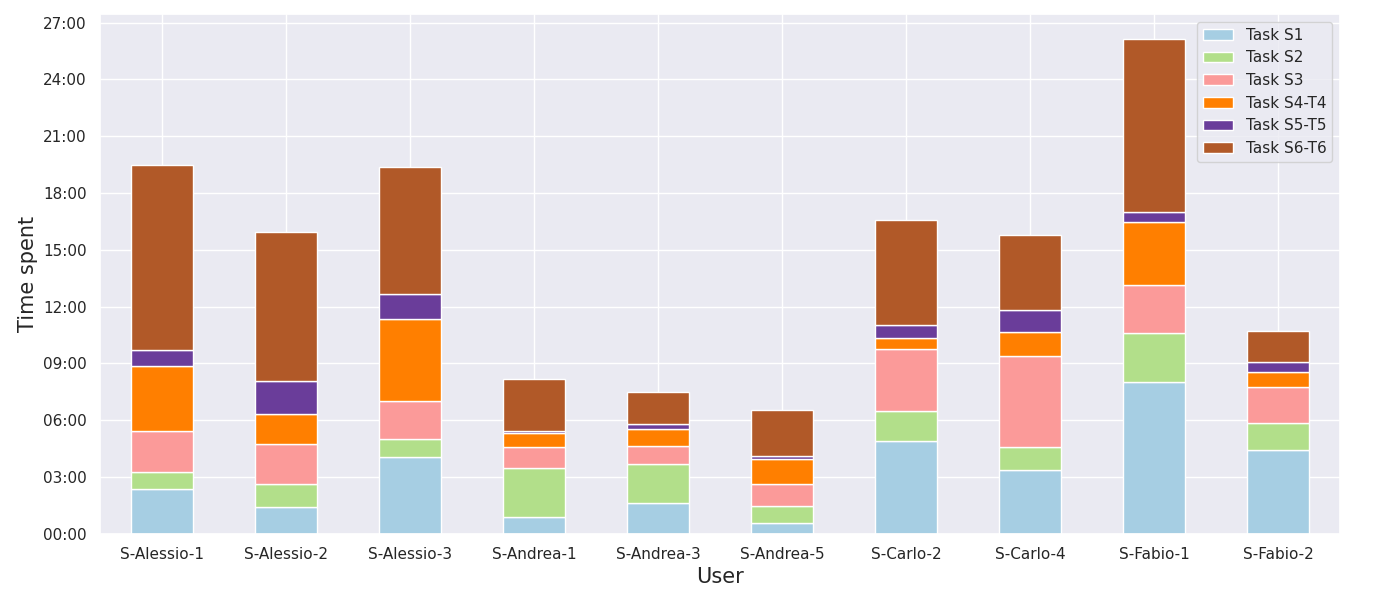
\includegraphics[width=1\textwidth]{images/ResultsEfficiencyStudent.png}}%
            \captionsetup{justification=centering}
            \caption{Time spent on each task for each student}
            \label{ResultsEfficiencyStudent}
        \end{minipage}
    \end{figure}
    \begin{figure}[!ht]
        \begin{minipage}{\linewidth}
            \centering
            \makebox[\textwidth][c]{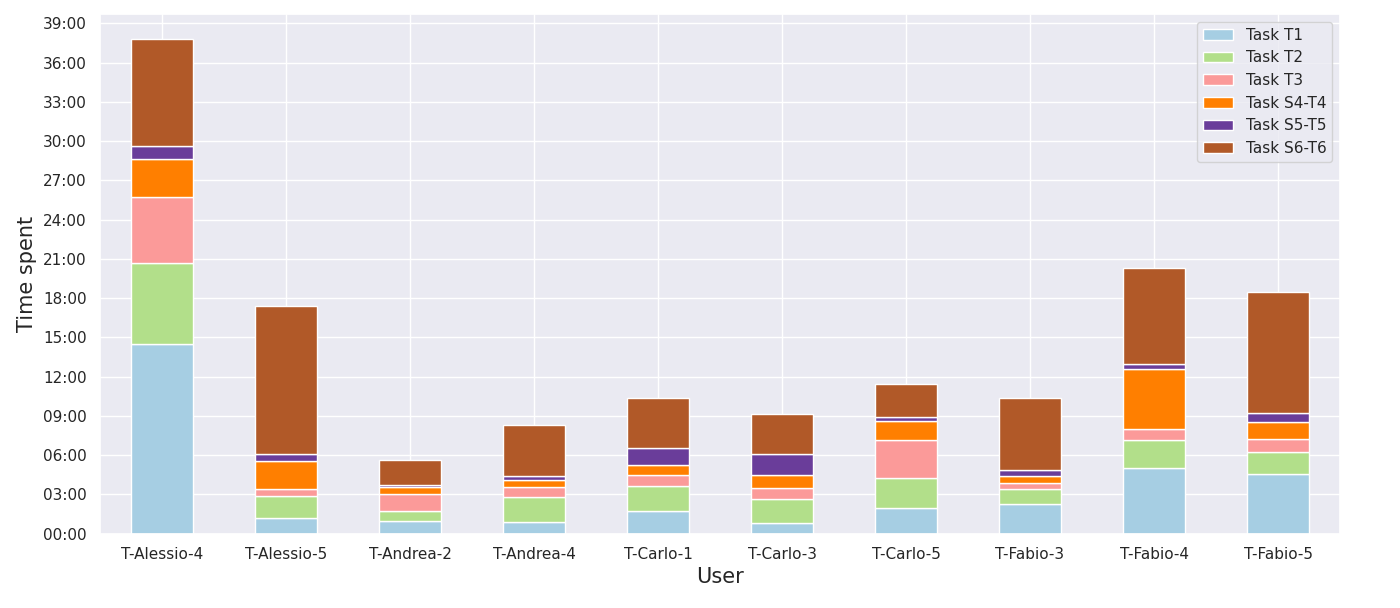
\includegraphics[width=1\textwidth]{images/ResultsEfficiencyTourist.png}}%
            \captionsetup{justification=centering}
            \caption{Time spent on each task for each tourist}
            \label{ResultsEfficiencyTourist}
        \end{minipage}
    \end{figure}


    \begin{figure}[!ht]
        \begin{minipage}{\linewidth}
            \centering
            \makebox[\textwidth][c]{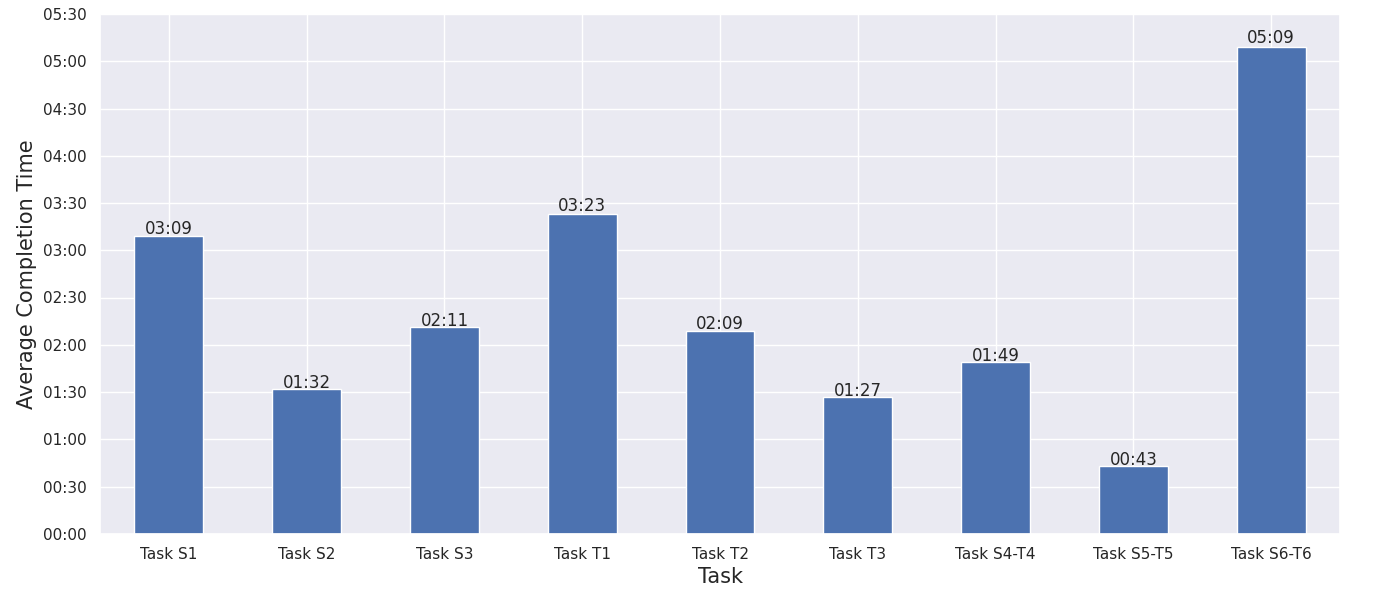
\includegraphics[width=1.1\textwidth]{images/ResultsEfficiencyAvg.png}}%
            \captionsetup{justification=centering}
            \caption{Average completion time for each task}
            \label{ResultsEfficiencyAvg}
        \end{minipage}
    \end{figure}

\pagebreak

\subsubsection{Errors}
    A summary graph in Fig. \ref{BarsErrors} shows the average of user errors for each task.
    \begin{figure}[!ht]
        \begin{minipage}{\linewidth}
            \centering
            \makebox[\textwidth][c]{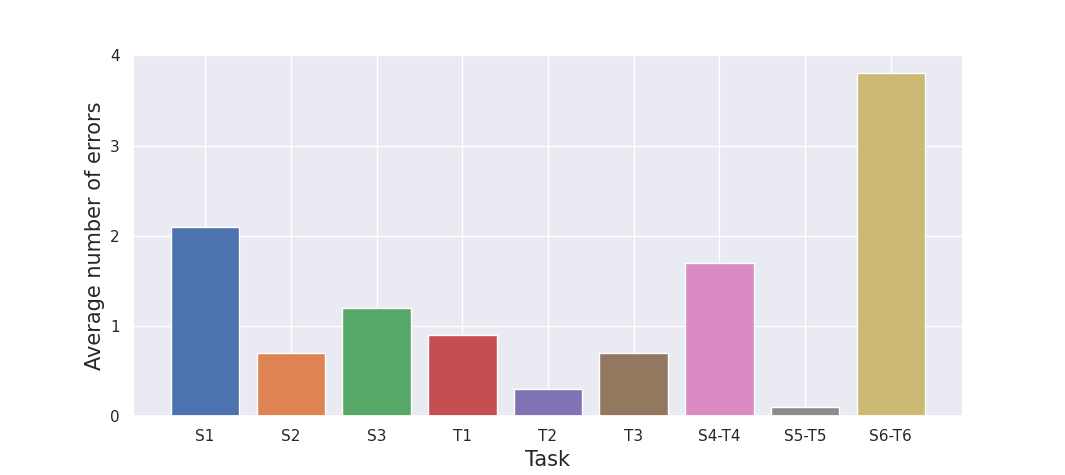
\includegraphics[width=1\textwidth]{images/BarsErrors.png}}%
            \captionsetup{justification=centering}
            \caption{Average of user errors for each task}
            \label{BarsErrors}
        \end{minipage}
    \end{figure}


\subsection{Discussion of results}
    % Your observations on results
    % Summary of comments from user testing
    Analyzing the graphs, as expected the users performed poorly on the task S6-T6. The task should not be very difficult, but due to the footer link "all the venues" missing in the main menu it underperformed. As a matter of fact, many it is also the task on which the users spent the most amount of time and committed the most amount of errors.\\
    On the other hand, the task S5-T5 regarding Covid has 100\% completion rate with almost zero errors: a link directly leading to the Covid page is immediately visible on the top of the home page.\\
    Finally, we summarize the various comments of the inspectors in the following points:
    \begin{itemize}
        \item The search bar was used more frequently than we thought so, but it had a negative impact on the user experience. Due to its slowness, many users were left waiting for a long period, wondering if it were a connection problem or not. Some of the users were frustrated and even gave up on the task, while the more patient ones were able to retrieve the queried information and were quite satisfied.
        \item Contrary to what we expected, many users did not notice immediately the main menu on the top right, which leads to confusion and disorientation in the first tasks. In addition, those who knew of its existence preferred to use the search bar.
        \item In many pages there are no searching filters or they're poor (e.g. must-see-attractions page, hotels main page). So the users can't find immediately what they're looking for, resulting in long wandering periods.
        \item Some important links (like "all the venues" mentioned above) are in the footer, so they're rarely seen and used. This leads to wandering periods and disorientation.
        \item The searching form in the restaurant page has some bugs (!!! IN FUTURO dire quali sono questi bug, perchè la pagina è cambiata. !!!). Thus, the website sometimes has an unexpected behavior, causing frustation in the users.
        \item The label "guide to the city" is misleading, in fact many users felt disoriented when they found that it does not lead to information about public transport.
    \end{itemize}